\documentclass[10pt]{beamer}

\usetheme[progressbar=frametitle]{metropolis}
\usepackage{appendixnumberbeamer}
\usepackage{pgfpages}
\usepackage{booktabs}
\usepackage{xcolor}
\usepackage{mathtools}

\usepackage{pgfplots}

\usepgfplotslibrary{dateplot}

\setbeameroption{slides only}
%\setbeameroption{show only notes}
%\setbeameroption{show notes on second screen=right}
\usepackage{xspace}
\newcommand{\themename}{\textbf{\textsc{metropolis}}\xspace}

\title{Labor Markets and Technological Change: Evidence from Electronic Health Records}

\subtitle{Hanna Glenn}
 \date{\today}

\setbeamertemplate{caption}{\raggedright\insertcaption\par}
\setbeamertemplate{itemize item}{\scalebox{.6}{$\blacktriangleright$ }}     
\setbeamertemplate{itemize subitem}{\scalebox{.8}{$\centerdot$ }} 

\begin{document}

\maketitle

\setbeamercolor{background canvas}{bg=white}



\section[Motivation]{Motivation}

\begin{frame}{The Broad Question}
\begin{itemize}
    \item Longstanding topic in economics: how does technology affect employment?
    \vspace{3mm}
    \item Been investigated in many industries
    \vspace{3mm}
    \item Specific healthcare setting
\end{itemize}

\note{An interesting and prominent question in economics is how technology affects employment and other labor market factors. This question has been studied for a long time and has entire chapters of books dedicated to it. People are generally very interested in how their jobs and the jobs of their children will be affected by technology. Empirically, this has been studied across sectors and industries and countries. In this paper, I am thinking about a very specific type of technology: electronic health records. }
\end{frame}

\begin{frame}[fragile]{What is an Electronic Health Record?}
At the least:
\begin{itemize}
    \item Switching from transcribing to computerization
\end{itemize}

\vspace{3mm}

More:
\begin{itemize}
    \item Communication
    \item Decision making assistance
\end{itemize}

\note[item]{So what actually are electronic health records? At their most basic, they computerize patient records that used to be kept on paper. For example, before EHRs a doctor would look at an ultrasound and they would talk into a microphone about what they saw. Then the recording would go to transcribers who record what the doctor said. So, when basic EHRs are implemented they record things directly into a computer instead of talking into a microphone. More complex systems have similar transitions. Systems can have messaging components that have transformed communication from letter writing to sitting down and hitting a few buttons. Another aspect you can imagine is a physician sitting down with a patient and receiving a popup on the screen that tells them the patient should have had a colonoscopy by now. So these systems change a lot about how physicians practice.}

\end{frame}

\begin{frame}[fragile]{HIT: Great (Expected) Potential in Healthcare}
\begin{alertblock}{Cost Saving}
\begin{itemize}
    \item Possible cost reduction of hundreds of billions of dollars \\ \scriptsize (Hillestad et al 2005)
\end{itemize}
\end{alertblock}

\begin{alertblock}{Quality Improvement}
\begin{itemize}
    \item Improved efficiency, patient safety improvements, physicians have decision support that could prevent unnecessary complications, etc.
    \item Significant policy push for EHR implementation: HITECH Act, 2008 provided financial incentive for hospitals to implement EHRs 
\end{itemize}
\end{alertblock}

\vspace{4mm}

\textcolor{blue}{The percentage of hospitals with basic EHR capability rose from 9$\%$ in 2008 to 84$\%$ in 2015.} \scriptsize (Health IT Dashboard)



\note[item]{\tiny Technology improvements in health to improve efficiency have been a huge deal. The reason for this is two-fold: the expected cost saving and the expected quality improvements.}
\note[item]{Before EHRs were standard, people expected the cost saving of these things to be massive. One study in particular estimated cost savings of hundreds of billions of dollars if HIT was fully implemented.}
\note[item]{In addition to the cost saving, the assumption was that new HIT would indirectly affect patient care/outcomes as well. Doctors could see more patients and faster, they have assistance to prevent unnecessary mistakes, etc.}
\note[item]{These expectations are what led to the incentivizing of using EHRs "meaningfully". All of these factors led to hospitals switching over to EHRs: 9 percent of hospitals with EHRs grew to 84 percent in 2015.}

\note[item]{Physicians are the primary users of the new technology. There is this stigma in healthcare about how difficult it has been for physicians to adjust to the new technologies. A main reason for this is the loss of autonomy and control a physician feels in their job. They go through all of this school just to have a computer tell them what to do?  But we don't know if physicians have changed their behavior in terms of labor market decisions. Since they are the bridge to the potential benefits of HIT and the realized benefits of HIT.}
\end{frame}


\begin{frame}[noframenumbering]{Physician Response to EHRs}
\begin{center}
    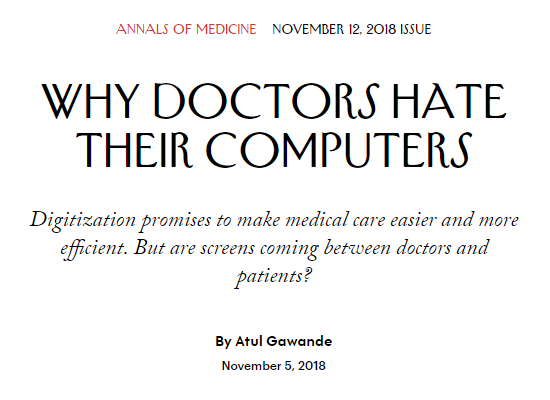
\includegraphics[scale=.5]{graphics/News Clip2.PNG}
\end{center}

\note[item]{I want to show you a couple examples of what is typical to see in the media about how physicians respond to EHRs. This headline is about how the very thing that is supposed to improve doctors' interactions with patients is the very thing causing compications.}
\end{frame}

\begin{frame}[noframenumbering]{Physician Response to EHRs}
\begin{center}
    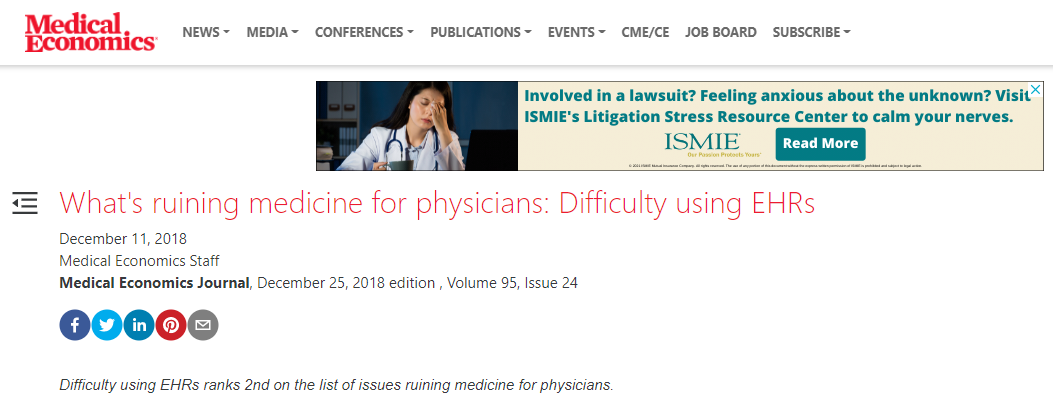
\includegraphics[scale=.35]{graphics/News Clip3.PNG}
\end{center}

\note[item]{Another headline here talks about EHRs ruining medicine for physicians. The subheading here says that this issue ranks 2nd in the list of issues ruining medicine for physicians. So do these technologies actually cause physicians to change their behavior? That is what I want to investigate.}
\end{frame}

\begin{frame}{This Paper}

Did EHR implementation in hospitals affect physician labor market decisions?
\begin{itemize}
    \item Intensive Margin / Productivity
    \item Extensive Margin
    \item Hospital $\rightarrow$ Office
\end{itemize}

\note[item]{This paper will specifically look at the effect of EHRs on physicians in three dimensions. First, on the intensive margin. Conditional on staying in the job, do EHRs lead to more or less patients being taken on? Second, on the extensive margin. Do EHRs lead physicians to actually retire early or leave their jobs? Third, I want to look at the work setting of the physician. Do EHRs in hospitals lead physicians to switch from hospital settings to office-based settings? Or transfer some of their workload to facilities in which they have more autonomy?}

\end{frame}


\section{Contribution}

\begin{frame}{Literature}
\small
\begin{columns}
\setlength{\tabcolsep}{-5pt}
    \column{0.33\textwidth}
        \centering
        \underline{ Technology $\rightarrow$ Labor }
        \vspace{-1mm}
        \begin{itemize}
            \item Erosion effect vs. wage effect \\ \vspace{1mm}
            \tiny (Zeira $\&$ Joseph 2011, EJ)
            
            \footnotesize
            
            \item Cause retirement? \\ \vspace{1mm}
            \tiny (Schleife 2006, Labour; Cavapozzi et al 2013, AE; Roger et al 2006, EJ; Friedburg 2003, ILRR)
            
            \footnotesize
            
            \item Older, well educated members of labor force exited at higher rates due to computerization \\ \vspace{1mm}
            \tiny (Willis and Hudomiet 2021, Labour)
        \end{itemize}
        
    \column{0.33\textwidth}
        \centering
        \color{gray}
        Physician Labor \underline{ Determinants }
        \vspace{-1mm}
        \begin{itemize}
        \color{gray}
            \item Physicians not very responsive to wage changes in terms of hours worked \\ \vspace{1mm}
            \tiny (Baltagi et al 2005, HE; Sloan 2018, ILRR)
            
            \footnotesize
            
            \item Personal life factors matter more for retirement than work conditions \\ \vspace{1mm}
            \tiny (Bahrami 2002, JHHSA)
            
            \footnotesize
            
            \item Physician burnout: early retirement and less hours worked \\ \vspace{1mm} 
            \tiny (Dewa et al 2014, BMC HSR)
        \end{itemize}
        
        \column{0.37\textwidth}
        \centering
        \color{gray}
        \underline{ EHR $\rightarrow$ Healthcare }
        \vspace{-1mm}
        \begin{itemize}
        \color{gray}
            \item Small improvements for severe health conditions \\ \vspace{1mm}
            \tiny(Agha 2014, JHE; McCullough et al 2016, RAND)
            
            \footnotesize
            
            \item Higher ``levels" of EHR use $\rightarrow$ decline in quality of care\\ \vspace{1mm}
            \tiny (Appari et al 2013, HSR)
            
            \footnotesize 
            
            \item No decrease in cost \\ \vspace{1mm}
            \tiny (Agha 2014, JHE; Dranove et al 2019, AEJ) 
            
            \footnotesize
            
            \item Productivity and opinion about EHRs varies drastically \\ \vspace{1mm}
            \tiny (Hitt $\&$ Tambe 2016, ILRR; Butler $\&$ Johnson 2016, IJHEM; Meyerhoefer et al 2016, ILRR)
            
        \end{itemize}
        
\end{columns}

\note[item]{\footnotesize Agha 2014 (JHE) uses claims data and difference in difference methodology. Find 1.3 percent increase in billed costs and no improvements in health coutcomes, data is 1998-2005.}

\note[item]{McCullough, Parente, Town 2016, RAND. claims data 2002-2007. Find no reduction in moretality for the median patient, only those who require complex care with coordination.}

\note[item]{Appari, Johnson, Anthony 2013. Health services review. fixed effects linear panel model. quality measure comes from hospital compare, not at the patient level.}

\note[item]{Dranove, Forman, Goldfarb, Greenstein (2019) American Economic Journal: Economic Policy. data from 1996 to 2009. Specific findings: hospitals have a rise in cost after 3 years, some hospitals in certain locations have a decrease in costs after 5 years but others still have a higher cost after 6 years.}

\end{frame}


\begin{frame}[noframenumbering]{Literature}
\footnotesize 
\small
\begin{columns}
\setlength{\tabcolsep}{-5pt}
    \column{0.33\textwidth}
        \centering
        \color{gray}
        \underline{ Technology $\rightarrow$ Labor }
        \vspace{-1mm}
        \begin{itemize}
        \color{gray}
            \item Erosion effect vs. wage effect \\ \vspace{1mm}
            \tiny (Zeira $\&$ Joseph 2011, EJ)
            
            \footnotesize
            
            \item Cause retirement? \\ \vspace{1mm}
            \tiny (Schleife 2006, Labour; Cavapozzi et al 2013, AE; Roger et al 2006, EJ; Friedburg 2003, ILRR)
            
            \footnotesize
            
            \item Older, well educated members of labor force exited at higher rates due to computerization \\ \vspace{1mm}
            \tiny (Willis and Hudomiet 2021, Labour)
        \end{itemize}
        
    \column{0.33\textwidth}
        \centering
        Physician Labor \underline{ Determinants }
        \vspace{-1mm}
        \begin{itemize}
            \item Physicians not very responsive to wage changes in terms of hours worked \\ \vspace{1mm}
            \tiny (Baltagi et al 2005, HE; Sloan 2018, ILRR)
            
            \footnotesize
            
            \item Personal life factors matter more for retirement than work conditions \\ \vspace{1mm}
            \tiny (Bahrami 2002, JHHSA)
            
            \footnotesize
            
            \item Physician burnout: early retirement and less hours worked \\ \vspace{1mm} 
            \tiny (Dewa et al 2014, BMC HSR)
        \end{itemize}
        
        \column{0.37\textwidth}
        \centering
        \color{gray}
        \underline{ EHR $\rightarrow$ Healthcare }
        \vspace{-1mm}
        \begin{itemize}
        \color{gray}
            \item Small improvements for severe health conditions \\ \vspace{1mm}
            \tiny(Agha 2014, JHE; McCullough et al 2016, RAND)
            
            \footnotesize
            
            \item Higher ``levels" of EHR use $\rightarrow$ decline in quality of care\\ \vspace{1mm}
            \tiny (Appari et al 2013, HSR)
            
            \footnotesize 
            
            \item No decrease in cost \\ \vspace{1mm}
            \tiny (Agha 2014, JHE; Dranove et al 2019, AEJ) 
            
            \footnotesize
            
            \item Productivity and opinion about EHRs varies drastically \\ \vspace{1mm}
            \tiny (Hitt $\&$ Tambe 2016, ILRR; Butler $\&$ Johnson 2016, IJHEM; Meyerhoefer et al 2016, ILRR)
            
        \end{itemize}
        
\end{columns}
\end{frame}

\begin{frame}[noframenumbering]{Literature}
\small
\begin{columns}
\setlength{\tabcolsep}{-5pt}
    \column{0.33\textwidth}
    \color{gray}
        \centering
        \underline{ Technology $\rightarrow$ Labor }
        \vspace{-1mm}
        \begin{itemize}
        \color{gray}
            \item Erosion effect vs. wage effect \\ \vspace{1mm}
            \tiny (Zeira $\&$ Joseph 2011, EJ)
            
            \footnotesize
            
            \item Cause retirement? \\ \vspace{1mm}
            \tiny (Schleife 2006, Labour; Cavapozzi et al 2013, AE; Roger et al 2006, EJ; Friedburg 2003, ILRR)
            
            \footnotesize
            
            \item Older, well educated members of labor force exited at higher rates due to computerization \\ \vspace{1mm}
            \tiny (Willis and Hudomiet 2021, Labour)
        \end{itemize}
        
    \column{0.33\textwidth}
        \centering
        \color{gray}
        Physician Labor \underline{ Determinants }
        \vspace{-1mm}
        \begin{itemize}
        \color{gray}
            \item Physicians not very responsive to wage changes in terms of hours worked \\ \vspace{1mm}
            \tiny (Baltagi et al 2005, HE; Sloan 2018, ILRR)
            
            \footnotesize
            
            \item Personal life factors matter more for retirement than work conditions \\ \vspace{1mm}
            \tiny (Bahrami 2002, JHHSA)
            
            \footnotesize
            
            \item Physician burnout: early retirement and less hours worked \\ \vspace{1mm} 
            \tiny (Dewa et al 2014, BMC HSR)
        \end{itemize}
        
        \column{0.37\textwidth}
        \centering
        \underline{ EHR $\rightarrow$ Healthcare }
        \vspace{-1mm}
        \begin{itemize}
            \item Small improvements for severe health conditions \\ \vspace{1mm}
            \tiny(Agha 2014, JHE; McCullough et al 2016, RAND)
            
            \footnotesize
            
            \item Higher ``levels" of EHR use $\rightarrow$ decline in quality of care\\ \vspace{1mm}
            \tiny (Appari et al 2013, HSR)
            
            \footnotesize 
            
            \item No decrease in cost \\ \vspace{1mm}
            \tiny (Agha 2014, JHE; Dranove et al 2019, AEJ) 
            
            \footnotesize
            
            \item Productivity and opinion about EHRs varies drastically \\ \vspace{1mm}
            \tiny (Hitt $\&$ Tambe 2016, ILRR; Butler $\&$ Johnson 2016, IJHEM; Meyerhoefer et al 2016, ILRR)
            
        \end{itemize}
        
\end{columns}
\end{frame}

\section{Data}

\begin{frame}{Data}
    Main data: \underline{CMS Shared Patient Data (2009-2015)}
    \begin{itemize}
        \item Hospital-physician pairs: bill for same patient
        \item Physician works in the hospital
    \end{itemize}
    EHR Use:
    \begin{itemize}
        \item Individual hospital EHR: AHA Survey
    \end{itemize}
    Other:
    \begin{itemize}
        \item Physician Compare
        \item Hospital Characteristics
    \end{itemize}
    
    \vspace{3mm}
    
    Aggregated to the physician level
\end{frame}


\begin{frame}{Variables}
Labor Market Outcomes:
\vspace{-2mm}
\begin{itemize}
    \item Patients visited in hospitals
    \item Maintaining billable activity only outside of hospitals
    \item \color{gray} Level of billable activity outside of hospitals
    \item \color{gray} Retirement/leaving the labor force
\end{itemize}

EHR Use:
\vspace{-2mm}
\begin{itemize}
    \item Indicator for any exposure to EHR
    \item \color{gray} Fraction of hospitals exposed to EHR
\end{itemize}

Other:
\vspace{-2mm}
\begin{itemize}
    \item Years of experience
    \item Hospital characteristics
\end{itemize}

\note[item]{So now we can talk }
\end{frame}


\begin{frame}{Data}
    \centering
    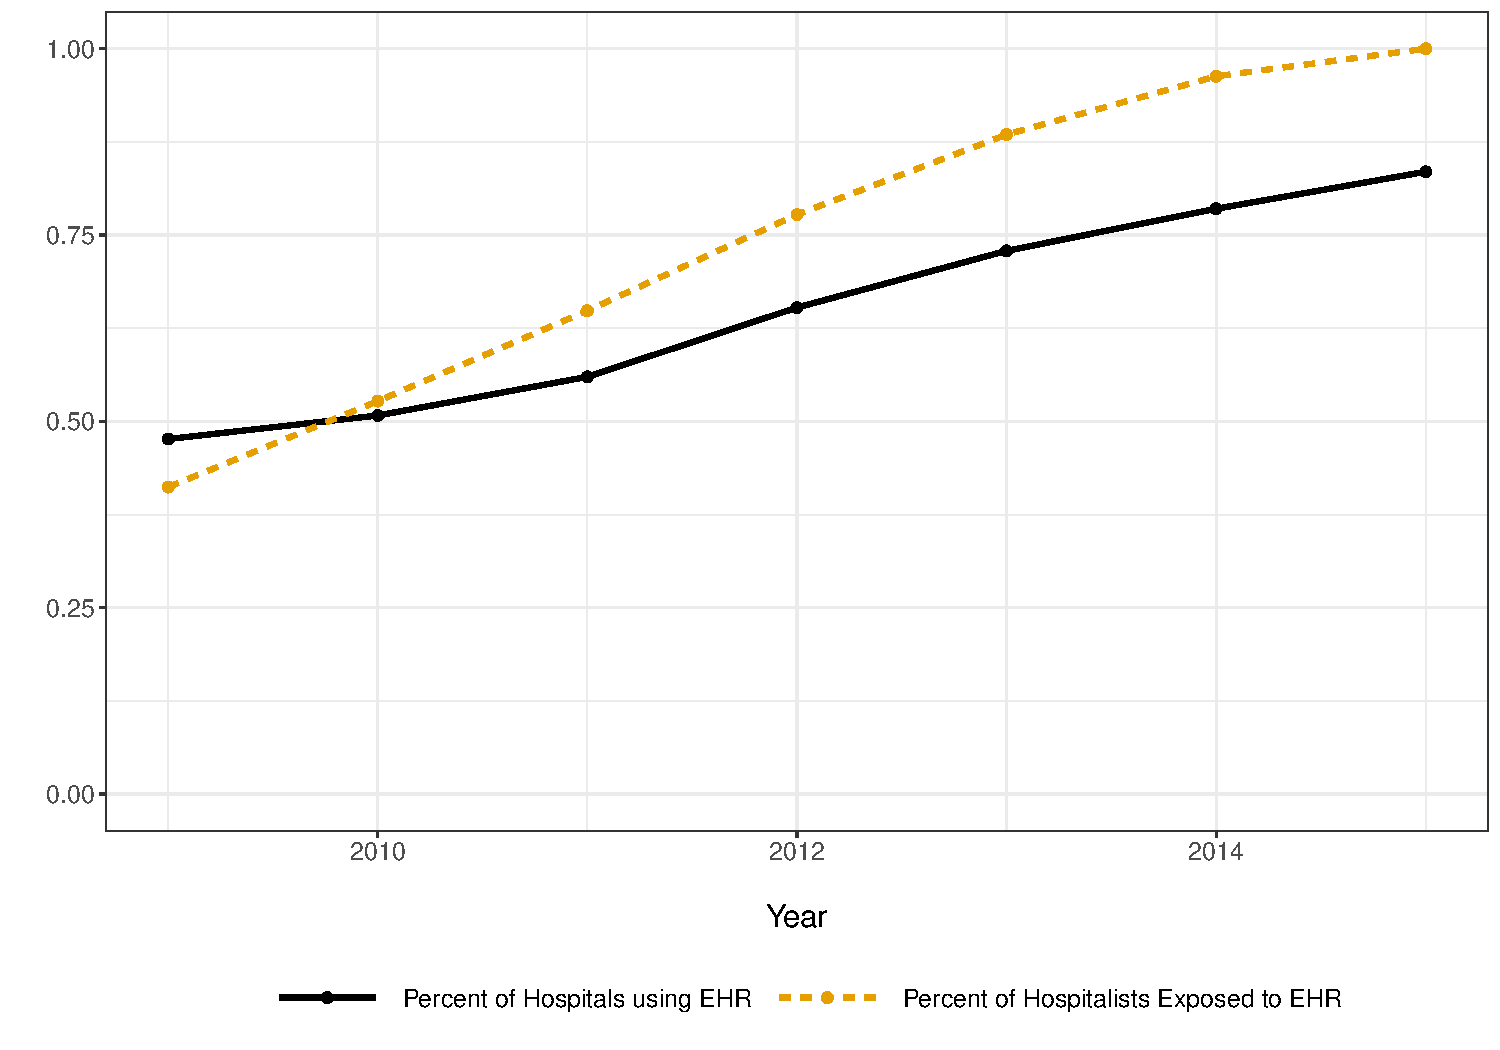
\includegraphics[scale=.5]{Objects/sum_stats_year.pdf}
\end{frame}

\begin{frame}{Data}
\centering
    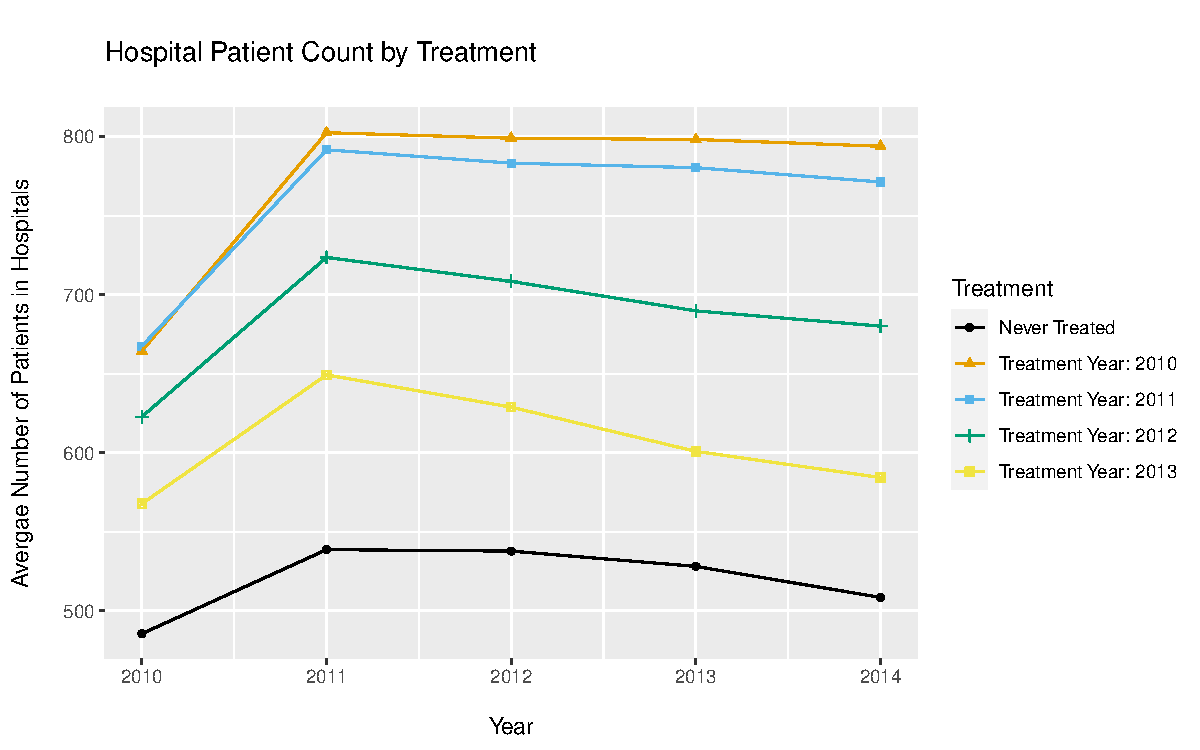
\includegraphics[scale=.5]{Objects/cont_treatment_graph.pdf}
    
\end{frame}

\begin{frame}{Data}
    \centering
    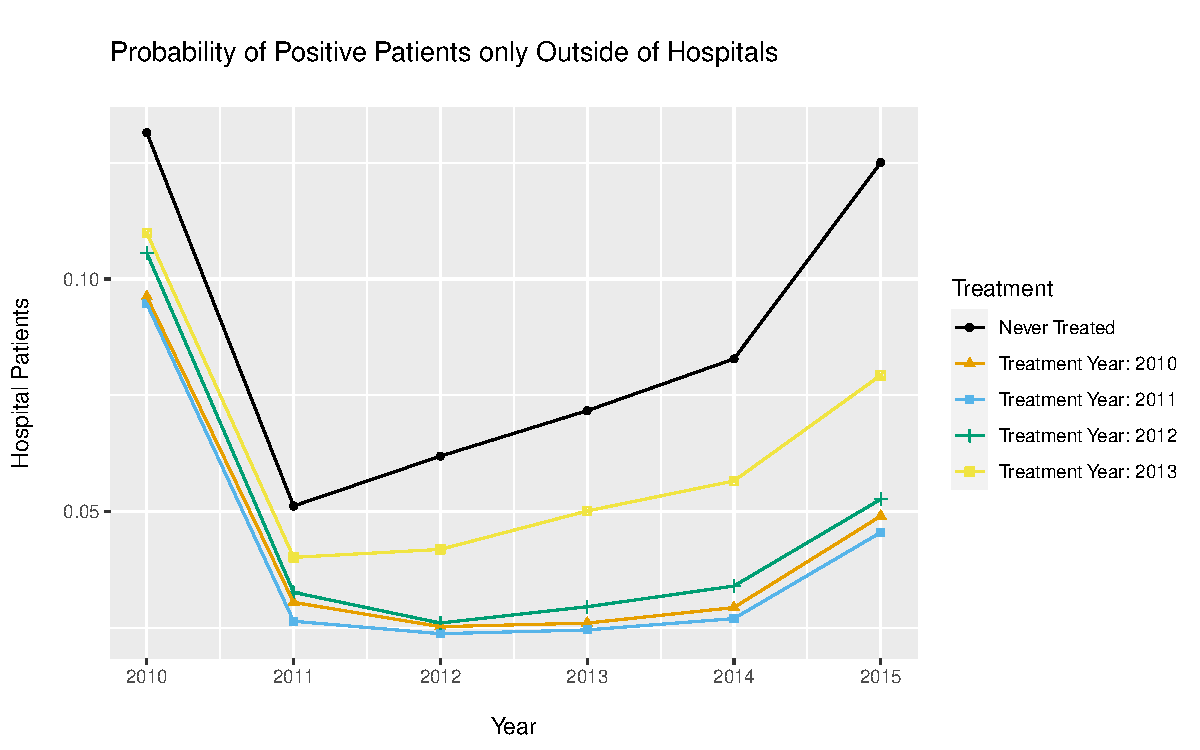
\includegraphics[scale=.5]{Objects/ind_treatment_graph.pdf}
\end{frame}




\section{Analysis}

\begin{frame}{Event Study}
\begin{equation*}
    y_{it}=\alpha_i+\delta_t+q_{it}'\lambda+\sum_{k=-5}^5 \beta_kz_{i,t-k} + \varepsilon_{it}
\end{equation*}

\vspace{4mm}

\begin{align*}
    y_{it} &: \text{Outcomes} \hspace{30mm}\\
    \alpha_i, \delta_t &: \text{Fixed Effects}\hspace{30mm}\\
    q_{it} &: \text{physician/hospital characteristics}\hspace{30mm}\\
    z_{i,t-k} &: \text{exposure to EHR} \hspace{30mm}
\end{align*}

    
\end{frame}

\section{Results}


\begin{frame}{Dep. Variable: Patients Billed with Hospitals}
\begin{figure}[ht]
        \begin{minipage}[b]{0.47\linewidth}
            \centering
            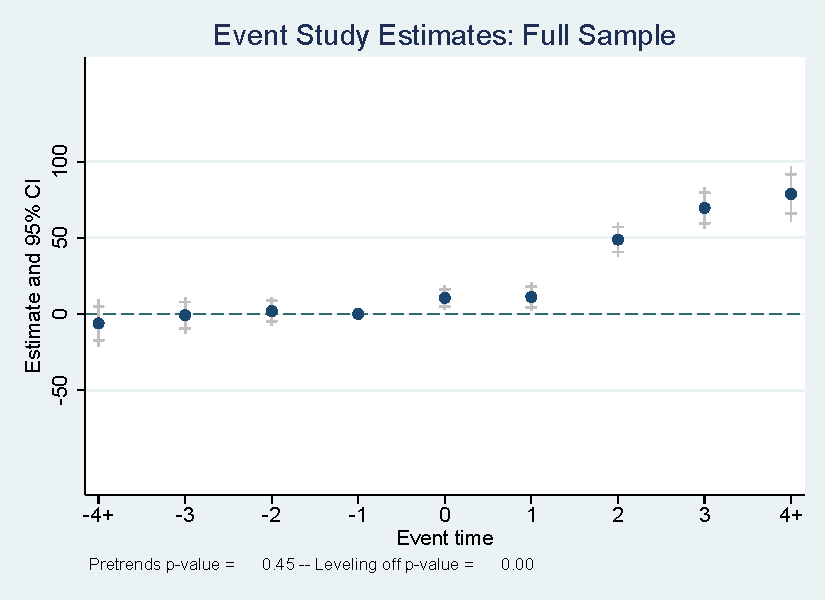
\includegraphics[width=\textwidth]{Objects/xtevent_fullsample.pdf}
            \caption{\small All Physicians\\}
        \end{minipage}
        \hspace{0.2cm}
        \begin{minipage}[b]{0.47\linewidth}
            \centering
            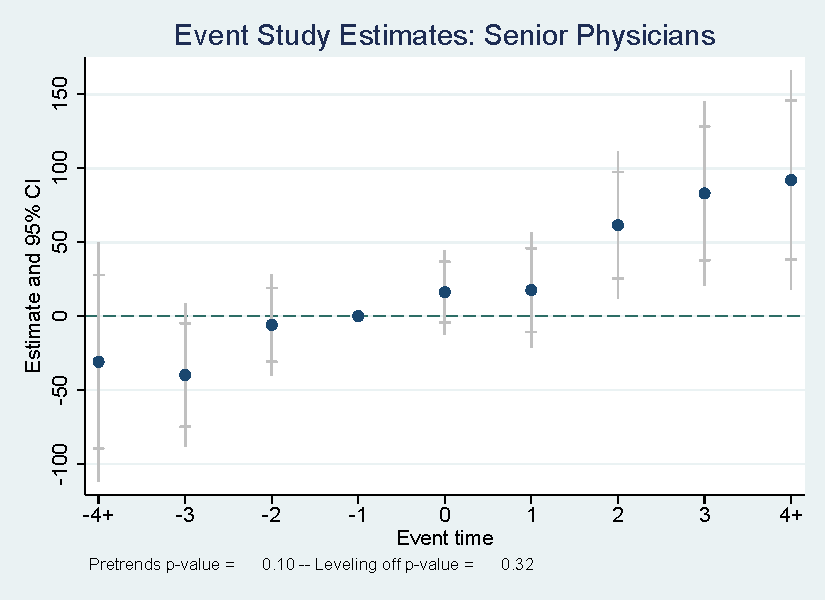
\includegraphics[width=\textwidth]{Objects/xtevent_oldsample.pdf}
            \caption{\small Phys. $>$ 35 yrs Experience}
        \end{minipage}
    \end{figure}
\end{frame}


\begin{frame}{Dep. Variable: Probability of Billing, but not With Hospitals}
\begin{figure}[ht]
        \begin{minipage}[b]{0.47\linewidth}
            \centering
            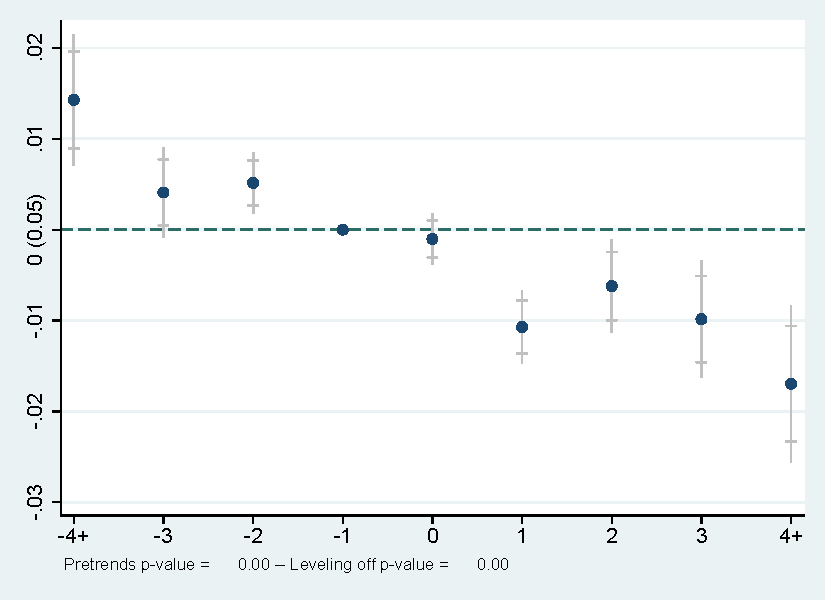
\includegraphics[width=\textwidth]{Objects/xtevent_fullsample_ind.pdf}
            \caption{\small All Physicians}
        \end{minipage}
        \hspace{0.2cm}
        \begin{minipage}[b]{0.47\linewidth}
            \centering
            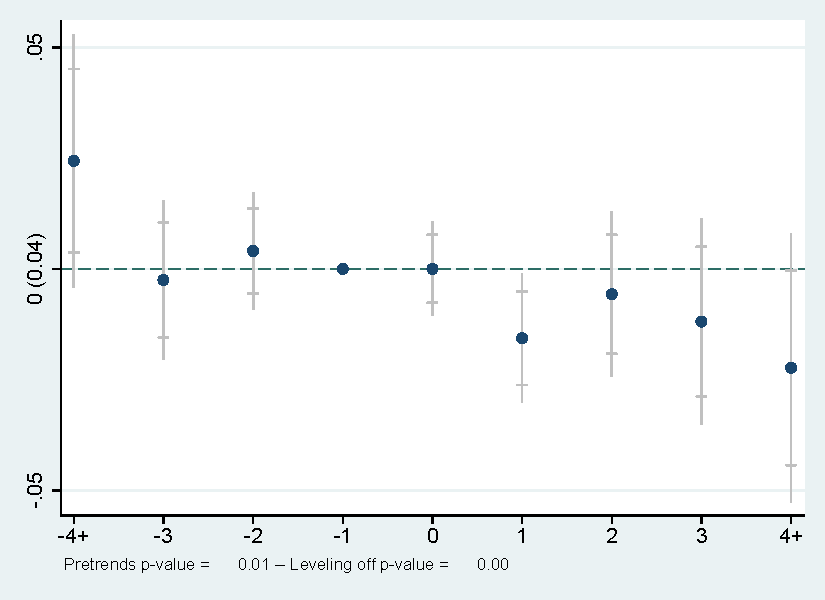
\includegraphics[width=\textwidth]{Objects/xtevent_oldsample_ind.pdf}
            \caption{\small Phys. $>$ 35yrs Experience}
        \end{minipage}
    \end{figure}
\end{frame}





\section{Continuing Work}

\begin{frame}{Plans}
    \begin{itemize}
        \item Analysis on retirement decision of physicians: requires a better understanding of why physicians would drop out of this Medicare data
        \item Investigate other estimation strategies
    \end{itemize}
\end{frame}

\begin{frame}{}
\centering
    Thank you!
\end{frame}



\end{document}
